\section{Proofs and Scope of the Guarantees}
\label{app:proofs}
\subsection{Measure-Theoretic Setup}
Let $AC^2([0,1];\M)$ denote absolutely continuous curves with square-integrable metric speed. The kernel in \cref{ass:paths} is measurable on continuous curves with their Borel sigma algebra and concentrated on $AC^2$. Let $\eta_{\mu,\nu}$ be its mixture under $\mu\otimes\nu$. We use a measurable version of the almost-everywhere tangent derivative under $\eta_{\mu,\nu}\otimes\dd s$; changing it on a product-null set does not change the discrepancy. Conditional tangent expectations can be constructed in measurable local orthonormal frames. Orthogonal changes of frame commute with conditional expectation, yielding an intrinsic field. Finite expected action gives square integrability under the folded time-observation law by Tonelli's theorem.

Write $R\gamma(s)=\gamma(1-s)$. Reversibility means $K_{y,x}=R_\#K_{x,y}$; its tangent version satisfies $(R\gamma)'(s)=-\dot\gamma(1-s)$ almost everywhere. Equality in law suffices. No globally smooth, unique logarithm is assumed.

\subsection{Proof of Theorem~\ref{thm:divergence}}
\begin{proof}
\emph{Finiteness and upper bound.} The normalized time density and equal-probability flip give
\begin{align}
\E_{t,B,\eta}\norm{g_{\gamma_s}}{\dot\gamma_s}^2
&=\int_0^{1/2}\E_\eta\big[\norm{g_{\gamma_t}}{\dot\gamma_t}^2
+\norm{g_{\gamma_{1-t}}}{\dot\gamma_{1-t}}^2\big]\dd t\notag\\
&=\E_\eta\int_0^1\norm{g_{\gamma_s}}{\dot\gamma_s}^2\dd s
=\mathcal A_\Gamma(\mu,\nu).
\end{align}
Conditional Jensen in each tangent fiber yields $0\leq\D_\Gamma^g\leq\mathcal A_\Gamma$.

\emph{Symmetry.} Swapping endpoints replaces the path law by its reversal. The transformation $(\gamma,B)\mapsto(R\gamma,1-B)$ preserves the selected point and negates its forward tangent velocity. Thus the observation law under $(\nu,\mu)$ is the same as under $(\mu,\nu)$, with conditional field $-m_t$. Its squared norm has the same expectation.

\emph{Zero on the diagonal.} If $\mu=\nu$, independent endpoints are exchangeable. The preceding transformation preserves the joint law of time and observation while negating $A_t$. Pairing against any bounded measurable tangent test field gives $\E g(h,A_t)=-\E g(h,A_t)=0$. Therefore $m_t=0$ almost everywhere and $\D_\Gamma^g(\mu,\mu)=0$.

\emph{Transport lower bound.} Take a smooth $\varphi$ with $\|\grad\varphi\|_g\leq1$. The chain rule along an absolutely continuous curve gives
\begin{equation}
\varphi(X_1)-\varphi(X_0)=\int_0^1g_{\gamma_s}(\grad\varphi(\gamma_s),\dot\gamma_s)\dd s.
\end{equation}
Finite action implies absolute integrability by Cauchy--Schwarz, justifying Fubini. Folding the interval and conditioning gives \cref{eq:fundamental}. Applying Cauchy--Schwarz under the resulting probability law yields
\begin{align}
\left|\E_\nu\varphi-\E_\mu\varphi\right|
&\leq\big(\E_t\E_{\bar\rho_t}\|\grad\varphi\|_g^2\big)^{1/2}
\sqrt{\D_\Gamma^g}\notag\\
&\leq\sqrt{\D_\Gamma^g}.
\end{align}
For a general $1$-Lipschitz potential, smooth Lipschitz approximation on a separable Riemannian manifold gives a uniform $\epsilon$-approximation with Lipschitz constant at most $1+\epsilon$ \citep{azagra2007smooth}. Apply the preceding estimate and let $\epsilon\downarrow0$. Finite first moments ensure finite endpoint expectations after subtracting a constant. Kantorovich--Rubinstein duality yields $W_1\leq\sqrt{\D_\Gamma^g}$. Since $W_1$ separates finite-first-moment measures, a zero discrepancy implies equal laws. For a constant-speed minimizing geodesic, its pathwise action is $d_g(X_0,X_1)^2$, proving the specialization.
\end{proof}

The lower and upper bounds do not require reversal symmetry. Reversibility supplies symmetry and the zero value on equal laws. Two Dirac endpoints joined by a constant-speed minimizing geodesic attain both bounds, so their constants are sharp. No probability density or global subtraction of endpoints appears in the proof.

\subsection{Continuity-Equation Interpretation}
For any smooth compactly supported vector field $h$, define the tangent current by $J_s(h)=\E_\eta g_{\gamma_s}(h(\gamma_s),\dot\gamma_s)$. Specializing to $h=\grad\varphi$ for smooth compactly supported scalar tests gives the weak equation $\partial_s\rho_s+\operatorname{div}_gJ_s=0$, where $\rho_s=\Law(\gamma_s)$. The folded observation satisfies
\begin{equation}
\bar\rho_t=(\rho_t+\rho_{1-t})/2,\qquad
\bar\rho_t m_t=(J_t+J_{1-t})/2.
\end{equation}
Hence $\partial_t(\rho_t-\rho_{1-t})=-2\operatorname{div}_g(\bar\rho_tm_t)$. If $m_t=0$, this difference is constant. It is zero at $t=1/2$ and equals $\mu-\nu$ at $t=0$, recovering definiteness. The current transporting $\bar\rho_t$ itself is $(J_t-J_{1-t})/2$; the discrepancy field and that transport velocity must not be conflated.

\subsection{Proof of Proposition~\ref{prop:variational}}
\begin{proof}
Conditioning on $(t,\widetilde X_t=x)$ replaces $A_t$ by $m_t(x)$ in the cross term. The identity $2g_x(f,m)-\|f\|_{g_x}^2=\|m\|_{g_x}^2-\|f-m\|_{g_x}^2$ proves the result. Finite action ensures integrability. Taking $f=m$ attains the supremum; a parameterized critic attains it only if it represents that conditional field up to observation-null sets.
\end{proof}

\subsection{Why the Guarantee Is Not a Wasserstein-2 Bound}
For linear paths on an interval $[0,L]$, let
\begin{equation}
\mu_a=\tfrac{1+a}{2}\delta_0+\tfrac{1-a}{2}\delta_L,\quad
\nu_a=\tfrac{1-a}{2}\delta_0+\tfrac{1+a}{2}\delta_L,
\end{equation}
where $a\in(0,1)$. Direct conditioning at the two moving observations gives
\begin{equation}
\D_\Gamma^g=\frac{2a^2L^2}{1+a^2},\qquad
W_1^2=a^2L^2,\qquad W_2^2=aL^2.
\end{equation}
Thus no universal $W_2^2\leq C\D_\Gamma^g$ holds, even on a bounded interval, as illustrated in \cref{fig:bounds}. This Euclidean example specifies the theorem's strength rather than a generation benchmark. On a domain of diameter $R$, $W_2^2\leq R W_1$ instead gives $W_2^2\leq R\sqrt{\D_\Gamma^g}$.

\subsection{Reversible Completion of Directed Paths}
\begin{proposition}
\label[proposition]{prop:symmetrize}
For a measurable finite-energy directed path law $K_{x,y}$ from $x$ to $y$, the kernel
\begin{equation}
\widehat K_{x,y}=\tfrac12K_{x,y}+\tfrac12R_\#K_{y,x}
\end{equation}
is reversible, preserves endpoints, and has action equal to the average of the two directed actions.
\end{proposition}
\begin{proof}
Use the involution $R_\#R_\#K=K$ to obtain $\widehat K_{y,x}=R_\#\widehat K_{x,y}$. Reversal preserves integrated squared speed and swaps endpoints, proving the other assertions.
\end{proof}
A corresponding implementation would sample another hidden orientation bit and use either a forward directed path or the reverse of a backward directed path, with the corresponding derivative sign. This is a construction recipe, not an evaluated branch of the present implementation. It retains the numerical solver's cost and does not supply gradients through a detached solver. A discretization additionally needs endpoint and reversal checks.

\subsection{Time Coverage, Boundaries, and Noise}
A single midpoint need not identify distributions for general reversible paths. On a short arc of $S^1$, connect angles $0$ and $a\in(0,\pi)$ by $\gamma_s=\exp(ia h(s))$, where $h(s)=1/2+4(s-1/2)^3$. This finite-energy path satisfies $h(1-s)=1-h(s)$ but has zero midpoint velocity. Distinct Dirac endpoints therefore have zero midpoint-only discrepancy. This example uses nonconstant speed and does not refute a theorem restricted to constant-speed geodesics.

Endpoint times themselves have zero sampling probability, but the full interval matters: restricting $t$ to $[\epsilon,1/2]$ identifies at most the interior laws $\rho_\epsilon$ and $\rho_{1-\epsilon}$. It does not justify equality of the original endpoints.

For a manifold with boundary, the path proof applies when curves remain inside, are absolutely continuous with finite action, and smooth Lipschitz approximation is valid for the intrinsic length metric. A current proof must hold for tests up to the boundary with no unaccounted source or sink. Interior-only continuity equations or final-output projection do not establish these conditions.

Random differentiable paths are already covered. A noisy interpolant must retain endpoints, reversal symmetry, finite action, and its \emph{full} time derivative. Perturbing a clean point and transporting only its clean velocity can retain cancellation while omitting noise-amplitude and exponential-map derivatives. Thus the deterministic theorem does not establish that noisy surrogate. For numerical targets, define
\begin{equation}
\epsilon^2=\E_{t\sim\mathcal U(0,1/2),B,\eta}\norm{g_{\widetilde X_t}}{\widehat A_t-A_t}^2,
\qquad \widehat m_t(x)=\E[\widehat A_t\mid t,\widetilde X_t=x],
\end{equation}
and $\widehat\D=\E_t\E_{\bar\rho_t}\|\widehat m_t\|_g^2$ under the same normalized law. Conditional Jensen gives $\|\widehat m-m\|_{L^2}\leq\epsilon$, and the triangle inequality implies $W_1\leq\sqrt{\widehat\D}+\epsilon$ for these same admissible observation paths.

\subsection{A Simulation-Free Randomized Torus Path}
\label{app:noisy-torus}
The following construction illustrates a noisy path whose actual derivative is available. On a flat $d$-torus, fix the shortest periodic displacement $\delta$ with a reversal-consistent tie rule. For $\xi\sim\mathcal N(0,I_d)$ independent of endpoints and fixed along the curve, set
\begin{align}
\gamma_s&=(x_0+s\delta+\varepsilon\sin(\pi s)\xi)\bmod2\pi,\notag\\
\dot\gamma_s&=\delta+\varepsilon\pi\cos(\pi s)\xi.
\label{eq:noisy-torus}
\end{align}
Both endpoints are exact. Using the same $\xi$ when reversing endpoints proves pathwise reversal symmetry, since $\sin(\pi(1-s))=\sin(\pi s)$ and the cosine derivative changes sign. Averaging the action over the independent Gaussian removes the cross term and yields
\begin{equation}
\mathcal A_\Gamma(\mu,\nu)=\E\|\delta\|_2^2+\frac{\varepsilon^2\pi^2d}{2}.
\end{equation}
This finite-energy randomized construction falls directly under \cref{thm:divergence}. It uses a differentiable random curve rather than a Brownian trajectory and needs no time-step simulation. Keeping only the clean displacement as target would be a different objective outside this particular proof. A mathematical construction alone does not establish that adding noise improves finite-network training.

\section{Geometric and Numerical Details}
\label{app:geometry}
For unit-sphere endpoints with $\alpha=\arccos(x^\top y)\in(0,\pi)$,
\begin{align}
\Log_x(y)&=\frac{\alpha}{\sin\alpha}(y-\cos\alpha\,x),\\
\Exp_x(v)&=x\cos\|v\|_2+v\frac{\sin\|v\|_2}{\|v\|_2}.
\end{align}
Small-angle limits avoid division by zero. Antipodes require a selected reversible great circle. Clipping an unstable logarithm is a numerical approximation, not a uniqueness result. The periodic displacement tie at $\pi$ on a torus has the same branch issue. Exact ties have probability zero for continuous endpoint laws, but near ties can still degrade numerical accuracy.

The SPD implementation uses the affine-invariant metric in \cref{eq:spd}, with matrix powers and logarithms from symmetric eigendecompositions. Cholesky diagonals are positive and a small jitter raises the spectrum; this fixed floor restricts the family. Log-Euclidean coordinates instead give a globally Euclidean geometry and do not test the affine-invariant metric tensor.

On the curvature-$-1$ Poincar\'e ball, $g_x(u,v)=\lambda_x^2u^\top v$ with $\lambda_x=2/(1-\|x\|_2^2)$. A radial map $0.995\tanh(\|h\|_2)h/\|h\|_2$ stays inside the numerical boundary. The legacy path code uses a central finite difference of radius $10^{-3}$, clamped at endpoint times, for its target velocity. These runs approximate the exact-path construction.

\section{Experimental Protocol and Result Provenance}
\label{app:protocol}
\subsection{Fixed Primary Protocol}
Model seeds are 0, 1, 2 and the fixed data-split seed is 0. MLPs have two hidden layers of width 128 (three affine layers), SiLU activations, and a 16-dimensional standard-normal latent. Critics and flow fields use eight Fourier time frequencies and raw wrapped spatial angles on tori. The kernel embedding used for evaluation is a separate circular embedding; it is not the critic input.
All runs use batch 256, float32, AdamW learning rate $2\times10^{-4}$ and weight decay zero. There is one critic update and one generator update per midpoint iteration. No neural-flow teacher is used. The mixture initialization is a train-fitted statistical starting model, not a pretrained flow. Torus mixtures use 64 components for General and 32 for other torsion datasets; sphere mixtures use 12 for Volcano and 24 otherwise. K-means initialization uses at most 8,192 training samples. Hard component selection leaves mixture-weight logits fixed during pathwise training; only centers and scales receive gradients.
The MMD control has the same constrained MLP output map and architecture as the MLP midpoint model and optimizes the biased batch MMD with the fixed training-reference kernel. It is an objective control, not an implementation of a kernel drifting algorithm. Every primary model is evaluated at prespecified steps; validation and test metrics are both saved but neither selects checkpoints or settings. Earlier test exposure is disclosed, so new metrics describe a locked evaluation on an already explored benchmark.
\subsection{Data Counts and Evaluation Size}
Table~\ref{tab:counts} records the local data counts and fixed evaluation size.
\begin{table}[t]\caption{Local preprocessing counts and fixed split sizes. The RNA count is 9,473; it is not asserted to equal every published preprocessing release.}\label{tab:counts}\centering\small\begin{tabular}{@{}lrrrrr@{}}\toprule
Data & Total & Train & Validation & Test & Evaluated $n$ \\
\midrule
Volcano & 827 & 663 & 82 & 82 & 82 \\
Earthquake & 6120 & 4896 & 612 & 612 & 612 \\
Flood & 4875 & 3901 & 487 & 487 & 487 \\
Fire & 12809 & 10249 & 1280 & 1280 & 1024 \\
General & 138208 & 110568 & 13820 & 13820 & 1024 \\
Glycine & 13283 & 10627 & 1328 & 1328 & 1024 \\
Proline & 7634 & 6108 & 763 & 763 & 763 \\
Pre-Pro & 6910 & 5528 & 691 & 691 & 691 \\
RNA (7D) & 9473 & 7579 & 947 & 947 & 947 \\
\bottomrule\end{tabular}\end{table}
All splits are by row. Molecular-source identifiers are not used for group splitting, and geographical rows can be dependent or duplicated. The conclusions concern the specified density-learning protocol, not unseen proteins, independent events, or temporal forecasting.
\subsection{Metrics}
For matched-size samples $x_{1:n}$ and $y_{1:n}$, the reported statistic is
\begin{equation}\widehat{\mathrm{MMD}}_V^2=\frac{1}{n^2}\sum_{i,j=1}^n\big[k(x_i,x_j)+k(y_i,y_j)-2k(x_i,y_j)\big].\end{equation}
The kernel denominator $h^2$ is the median strictly positive squared embedded distance among a fixed random training reference of at most 1,024 points. It is not fitted to generated or test samples. The diagonal terms are included, making this a biased V-statistic with a finite-sample floor; it is not an unbiased estimate. Test and validation targets are sampled without replacement using fixed independent target-selection seeds and reused across models and training seeds.
Nearest-neighbor distances use spherical angles and wrapped Euclidean angle distance on a flat torus. Spherical vectors are normalized in float64 and their angle is computed as $2\operatorname{atan2}(\|\hat x-\hat y\|_2,\|\hat x+\hat y\|_2)$, avoiding false positive distances between identical float32 directions. Symmetric NN is one half the sum of the two directed mean nearest distances. Coverage is the fraction of fixed target points within radius $r$ of a generated point; $r$ is the median positive leave-one-out nearest distance on the fixed training reference. Identical normalized directions are explicitly excluded from the sphere reference calibration. Mesh distances below are ambient Euclidean, not intrinsic geodesic distances.
Three generated draws are averaged within each training seed, followed by mean and sample standard deviation across the three independent training seeds. Draws are Monte Carlo replicates, not extra training seeds. Sphere validity is mean absolute unit-norm error. Torus validity is the fraction outside the half-open angle interval $[0,2\pi)$.
\subsection{Sampling and Compute}
The controlled RFM uses projected/exponential Euler with midpoint-in-time evaluation and one actual vector-field call per step. Both 1- and 128-NFE cases are saved at each prespecified checkpoint. Forward hooks verify counts. CUDA is synchronized around timing; GPU warmups and metric calculations are excluded. Single-thread CPU timing uses three repeated batches. Data preparation and mixture initialization are separately recorded, and training duration excludes evaluation pauses. This is not a claim of identical training FLOPs or total wall-clock cost across algorithms.
The final controlled bundle contains 72 completed training jobs, with 17.03 minutes of summed synchronized training time. This sum excludes evaluation, setup, discarded preliminary reruns, exploratory historical jobs, and incomplete attempts; it is not total project GPU time. Hardware: one NVIDIA GeForce RTX 4090, PyTorch 2.5.1 with CUDA 12.1. Other GPU processes were observed during part of this bundle; synchronized durations are actual wall times, not isolated hardware costs or proof of a speedup. Individual runs record their own durations.
\subsection{Randomness and Metric Audit}
A timing-helper audit exposed evaluation-induced resetting of a global CUDA stream in the preliminary GMM/RFM runs. The final bundle replaces all 54 affected runs using frozen sources and separate target, latent, time/flip, and flow-base RNG streams derived from model seed. It copies the 18 unaffected MLP objective-control jobs with file hashes. Evaluation is asserted to preserve all training streams at every checkpoint. Rerun checkpoints save optimizer and CPU/CUDA/private RNG states; the copied earlier MLP checkpoints are suitable for reevaluation but lack full continuation state. GPU reductions are not guaranteed bitwise identical across devices.
A separate analysis-only correction recomputes sphere angles and coverage from saved arrays with the normalized float64 metric above. Raw metric JSONs are archived with correction hashes, and training sources and generated arrays are unchanged. The final-table marker requires the corrected metric version. Both audits precede the final aggregation; neither selects models by their test scores.
\subsection{Reproduction Commands}
From the repository root with the provided conda environment, the following commands check and render the final recorded bundle. The experiment README gives the ordered training, immutable-snapshot rerun, metric-correction, and validation-only commands for a clean reconstruction.
\begingroup\small\begin{verbatim}
python paper/experiments/verify_independent.py
python paper/check_geometry.py
python paper/make_illustrations.py
python paper/update_results.py --run-root controlled_independent --require-complete
powershell -File paper/build.ps1
\end{verbatim}\endgroup
Data/split hashes and executed-code hashes accompany the final result ledger. Natural Earth public-domain land outlines are used only as geographic context in maps; density color fields are computed from saved samples.
Display KDEs are separate from the evaluation MMD kernel. Spherical plots use a normalized von Mises--Fisher kernel with concentration 45 (density per steradian); torus plots smooth a 120-by-120 periodic histogram using Gaussian sigma 2.4 bins and divide by angular bin area (density per squared radian). Comparisons use one logarithmic color scale and clip values below $10^{-3}$ of the maximum within that comparison. Horizontal geographic and angle domains span $[-180,180]$ degrees; only the first two RNA angles are displayed.

\section{Validation-Only Optimization Diagnostics}
\label{app:stability}
This post hoc diagnostic was motivated by the primary failures. It uses General training data and its fixed validation target only, model seed 0, and three generated draws per probe. No new test score is obtained or used to choose a candidate. Trials are reported together rather than replacing the unsuccessful primary setting. These exploratory results do not establish cross-seed robustness.
Table~\ref{tab:stability} records the initial and final validation outcomes.
\begin{table}[t]\caption{Validation-only General optimization study. All values are means of three Monte Carlo draws from one seed-0 model, not independent training replicates. MMD columns are multiplied by $10^3$; optimizer counts include critic warmup.}\label{tab:stability}\centering\small
\begin{tabular}{@{}llrrrrr@{}}\toprule
Configuration & Generator LR & Gen./field steps & Total updates & Initial val. & Final val. & Train s \\
\midrule
Raw random MLP, C=5 & 1e-05 & 2000 & 12500 & 750.34 & 256.37 & 19.8 \\
Periodic random MLP, C=5 & 1e-05 & 2000 & 12500 & 750.34 & 292.37 & 20.6 \\
Periodic random GMM, C=5 & 1e-05 & 2000 & 12500 & 203.86 & 199.85 & 20.8 \\
Periodic train-fit GMM, C=5 & 1e-05 & 2000 & 12500 & 0.82 & 0.83 & 20.7 \\
Periodic random MLP, C=10 & 1e-05 & 2000 & 22500 & 750.34 & 298.39 & 34.9 \\
Periodic RFM & 2e-04 & 22500 & 22500 & 195.40 & 1.91 & 30.4 \\
Periodic random MLP, C=5 & 2e-04 & 10000 & 60500 & 750.34 & 34.91 & 164.3 \\
Periodic random GMM, C=5 & 2e-04 & 10000 & 60500 & 203.86 & 16.40 & 171.0 \\
Periodic random MLP, C=5 & 1e-04 & 2000 & 12500 & 750.34 & 40.23 & 20.7 \\
Periodic random MLP, C=5 & 2e-04 & 2000 & 12500 & 750.34 & 35.00 & 20.8 \\
\bottomrule\end{tabular}\end{table}
The periodic critic/field uses sine and cosine spatial harmonics 1--4, eight Fourier time frequencies, width 128, and three affine layers. The study adds 500 critic-only warmup updates, five or ten critic updates per generator iteration, and slower generator learning rates, with the higher-rate refinement recorded separately. Its flow control uses the same periodic field architecture and fixed update counts; it must not be confused with the raw-angle controlled RFM in the primary table.
Figure~\ref{fig:stability} shows illustrative configurations from this post hoc study.
\begin{figure}[t]\centering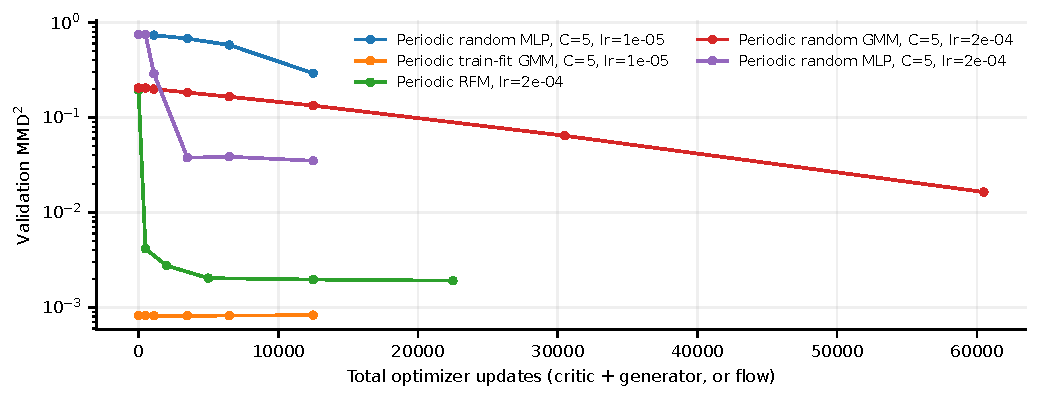
\includegraphics[width=\textwidth]{figures/validation_stability.pdf}
\caption{General validation diagnostics from one training seed. Lines join fixed probe checkpoints; they are not interpolated test estimates. Curves illustrate retention, random initialization, higher-rate refinement, and periodic RFM; all completed trial outcomes are listed in Table~\ref{tab:stability}. Update counts are not equal FLOPs; measured training times appear in the table.}\label{fig:stability}\end{figure}

\subsection{True-Velocity Randomized Paths}
We separately probe the reversible randomized torus path in \cref{eq:noisy-torus} on General, with $\varepsilon\in\{0,0.3,0.7\}$. The actual derivative includes the noise-amplitude derivative. The experiment uses a randomly initialized MLP, the periodic critic, seed 0, batch 512, 10,000 generator updates, five critic updates per generator step, 500 critic warmup updates, and generator/critic learning rates $2\times10^{-4}$. All three amplitudes and fixed checkpoints are specified before this diagnostic. It is post hoc validation-only evidence, not a replacement for the primary table or independent-seed confirmation. Evaluation preserves the training RNG state.
Table~\ref{tab:noise} lists every amplitude. Figure~\ref{fig:noise} shows the fixed-checkpoint validation curves. The $\varepsilon=0$ row is a separately executed deterministic control with the same code path and random draws, not a copied earlier result.
\begin{table}[t]\caption{Randomized-torus validation diagnostic. One seed-0 model per amplitude; MMD$^2\times10^3$ means average three sampling draws. The final SD is Monte Carlo variation only. No test metrics are evaluated.}\label{tab:noise}\centering\small\begin{tabular}{@{}rrrrr@{}}\toprule
Amplitude $\varepsilon$ & Initial val. & Final val. & Final MC SD & Train s \\
\midrule
0 & 750.34 & 60.70 & 3.86 & 159.9 \\
0.3 & 750.34 & 36.53 & 1.85 & 156.0 \\
0.7 & 750.34 & 31.68 & 0.71 & 150.2 \\
\bottomrule\end{tabular}\end{table}
Noise improves the final validation MMD relative to this deterministic control in the single-seed sweep, but all three models remain above the periodic RFM reference (approximately $1.91\times10^{-3}$). Their 60,500 total optimizer updates exceed that reference's 22,500 field updates; neither update counts nor FLOPs are matched. This diagnostic does not establish cross-seed efficacy or an advantage over the flow.
\begin{figure}[t]\centering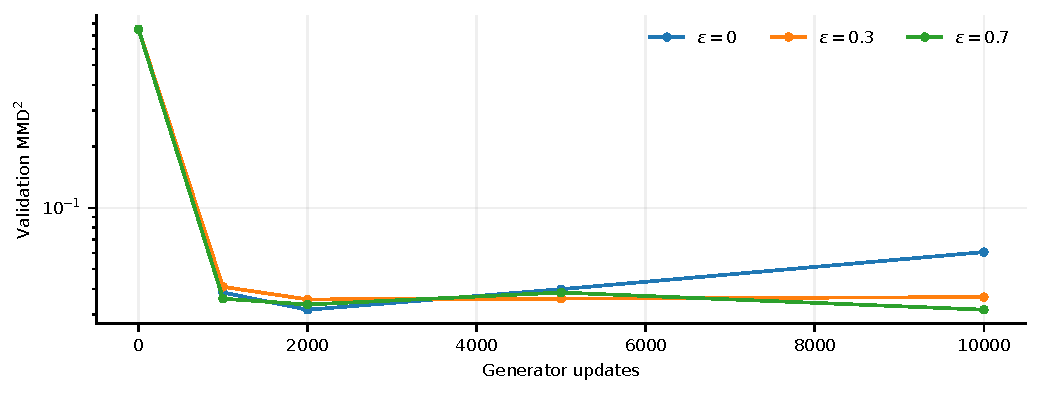
\includegraphics[width=\textwidth]{figures/validation_noise.pdf}
\caption{Validation-only true-velocity noise diagnostic. Lines join prespecified checkpoints for three seed-0 models. Different amplitudes define different path discrepancies; these curves do not estimate the population divergence or establish a generally optimal noise level.}\label{fig:noise}\end{figure}

\clearpage
\section{Additional Quantitative and Qualitative Results}
\label{app:additional}
\begin{figure}[t]
\centering
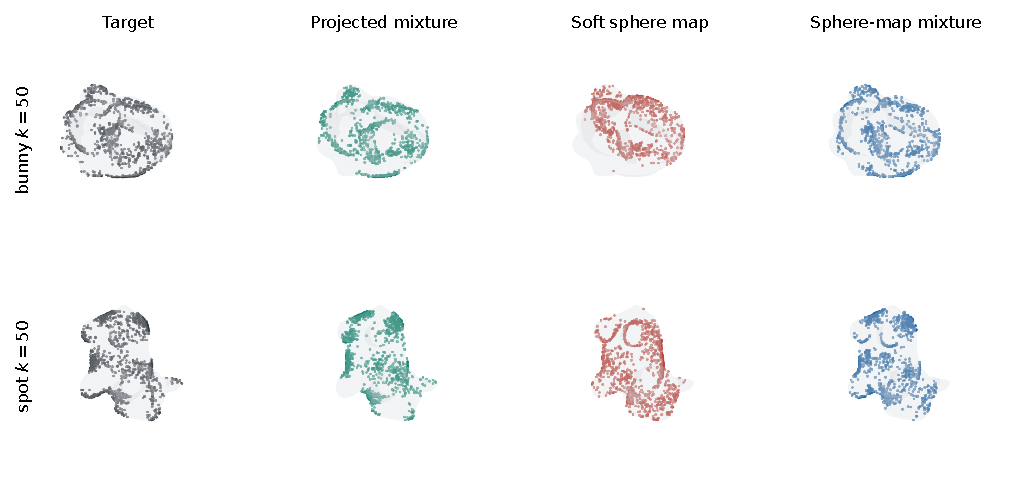
\includegraphics[width=\textwidth]{figures/mesh_selected.pdf}
\caption{\textbf{Exploratory surface generation.} Fixed final checkpoints on Bunny $k=50$ and Spot $k=50$, with identical cameras and 1,024 points in each panel. Columns show target samples and three constrained-generator variants. All use the local projected-chord surrogate; the soft sphere map is not a certified bijection. Qualitative resemblance and output validity do not establish agreement of intrinsic densities.}
\label{fig:mesh}
\end{figure}
\subsection{Full Sample Metrics}
Table~\ref{tab:all-metrics} supplements Table~\ref{tab:main} with distances, coverage, and validity.
\begin{table}[t]\caption{Additional controlled test metrics, mean $\pm$ training-seed SD for NN and coverage. Validity reports the mean error defined in the text.}\label{tab:all-metrics}\centering\small\begin{tabular}{@{}llrrr@{}}\toprule
Data & Method / updates & Symmetric NN $\downarrow$ & Coverage $\uparrow$ & Validity error $\downarrow$ \\
\midrule
Volcano & R-MGM mixture / 2k & $0.119\,\pm\,0.021$ & $0.028\,\pm\,0.019$ & $3.0e-08$ \\
Volcano & RFM / 2k & $0.204\,\pm\,0.003$ & $0.005\,\pm\,0.006$ & $3.3e-08$ \\
Volcano & RFM / 10k & $0.189\,\pm\,0.003$ & $0.005\,\pm\,0.005$ & $3.5e-08$ \\
Earthquake & R-MGM mixture / 2k & $0.044\,\pm\,0.001$ & $0.156\,\pm\,0.006$ & $3.2e-08$ \\
Earthquake & RFM / 2k & $0.101\,\pm\,0.000$ & $0.054\,\pm\,0.003$ & $3.5e-08$ \\
Earthquake & RFM / 10k & $0.079\,\pm\,0.001$ & $0.092\,\pm\,0.009$ & $3.5e-08$ \\
Flood & R-MGM mixture / 2k & $0.052\,\pm\,0.001$ & $0.123\,\pm\,0.022$ & $3.0e-08$ \\
Flood & RFM / 2k & $0.097\,\pm\,0.001$ & $0.062\,\pm\,0.004$ & $3.4e-08$ \\
Flood & RFM / 10k & $0.087\,\pm\,0.001$ & $0.073\,\pm\,0.012$ & $3.4e-08$ \\
Fire & R-MGM mixture / 2k & $0.028\,\pm\,0.002$ & $0.144\,\pm\,0.015$ & $3.0e-08$ \\
Fire & RFM / 2k & $0.087\,\pm\,0.001$ & $0.022\,\pm\,0.000$ & $3.5e-08$ \\
Fire & RFM / 10k & $0.067\,\pm\,0.002$ & $0.035\,\pm\,0.001$ & $3.4e-08$ \\
General & R-MGM mixture / 2k & $0.096\,\pm\,0.019$ & $0.198\,\pm\,0.092$ & $0.0e+00$ \\
General & RFM / 2k & $0.166\,\pm\,0.001$ & $0.203\,\pm\,0.010$ & $0.0e+00$ \\
General & RFM / 10k & $0.132\,\pm\,0.001$ & $0.269\,\pm\,0.006$ & $0.0e+00$ \\
Glycine & R-MGM mixture / 2k & $0.172\,\pm\,0.033$ & $0.091\,\pm\,0.043$ & $0.0e+00$ \\
Glycine & RFM / 2k & $0.161\,\pm\,0.002$ & $0.118\,\pm\,0.004$ & $0.0e+00$ \\
Glycine & RFM / 10k & $0.114\,\pm\,0.003$ & $0.238\,\pm\,0.006$ & $0.0e+00$ \\
Proline & R-MGM mixture / 2k & $0.136\,\pm\,0.011$ & $0.064\,\pm\,0.029$ & $0.0e+00$ \\
Proline & RFM / 2k & $0.230\,\pm\,0.002$ & $0.104\,\pm\,0.012$ & $0.0e+00$ \\
Proline & RFM / 10k & $0.101\,\pm\,0.007$ & $0.213\,\pm\,0.014$ & $0.0e+00$ \\
Pre-Pro & R-MGM mixture / 2k & $0.061\,\pm\,0.016$ & $0.316\,\pm\,0.062$ & $0.0e+00$ \\
Pre-Pro & RFM / 2k & $0.157\,\pm\,0.002$ & $0.204\,\pm\,0.006$ & $0.0e+00$ \\
Pre-Pro & RFM / 10k & $0.134\,\pm\,0.004$ & $0.246\,\pm\,0.026$ & $0.0e+00$ \\
RNA (7D) & R-MGM mixture / 2k & $0.396\,\pm\,0.002$ & $0.314\,\pm\,0.010$ & $0.0e+00$ \\
RNA (7D) & RFM / 2k & $0.965\,\pm\,0.004$ & $0.000\,\pm\,0.000$ & $0.0e+00$ \\
RNA (7D) & RFM / 10k & $0.736\,\pm\,0.013$ & $0.041\,\pm\,0.015$ & $0.0e+00$ \\
\bottomrule\end{tabular}\end{table}
Spherical NN units are radians. Torus NN uses the Euclidean norm of wrapped angular differences in radians. The coverage threshold is fixed separately per dataset from training data. Validity means unit-norm error on a sphere and out-of-range fraction on a torus; these different quantities must not be averaged across domains.
\subsection{Matched MLP Objective Controls}
Figure~\ref{fig:objective-controls} visualizes the parameterization-matched models from training seed 0.
\begin{figure}[t]\centering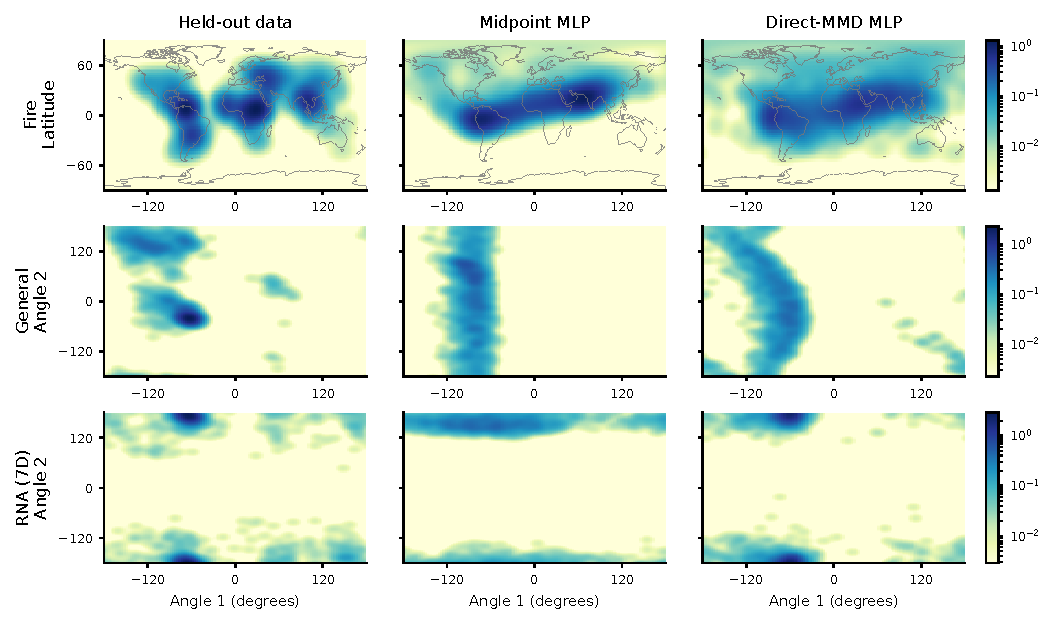
\includegraphics[width=\textwidth]{figures/objective_controls.pdf}
\caption{Matched constrained MLPs after 2,000 updates: the same fixed test targets and training seed 0, with midpoint and direct-MMD objectives. Each row uses one logarithmic KDE scale and the plotting convention of Figure~\ref{fig:controlled}. Only the first two RNA angles are displayed. These are sample densities, not model likelihoods.}\label{fig:objective-controls}\end{figure}
Table~\ref{tab:mlp-metrics} supplements the matched-architecture objective comparison with non-MMD metrics. The MMD control directly optimizes the evaluation kernel, so its MMD advantage alone would not establish superiority on all distributional criteria.
\begin{table}[t]\caption{Matched MLP controls at 2,000 generator updates. Mean and sample SD across three training seeds, after averaging three draws per seed. Smaller symmetric NN and larger coverage are better.}\label{tab:mlp-metrics}\centering\small\begin{tabular}{@{}llrr@{}}\toprule
Data & Objective & Symmetric NN & Coverage \\
\midrule
Fire & Midpoint & $0.115\,\pm\,0.011$ & $0.024\,\pm\,0.017$ \\
Fire & Direct MMD & $0.080\,\pm\,0.002$ & $0.030\,\pm\,0.004$ \\
General & Midpoint & $0.168\,\pm\,0.022$ & $0.196\,\pm\,0.026$ \\
General & Direct MMD & $0.158\,\pm\,0.004$ & $0.257\,\pm\,0.011$ \\
RNA (7D) & Midpoint & $0.913\,\pm\,0.225$ & $0.000\,\pm\,0.000$ \\
RNA (7D) & Direct MMD & $0.508\,\pm\,0.016$ & $0.111\,\pm\,0.039$ \\
\bottomrule\end{tabular}\end{table}
\subsection{Numerical Geometry Audits}
Table~\ref{tab:geometry-audit} reports the interpolation residuals.
\begin{table}[t]\caption{Maximum numerical residuals over 64 float64 endpoint pairs per geometry. Position and derivative-comparison norms are ambient; velocity reversal uses the manifold metric.}\label{tab:geometry-audit}\centering\small\begin{tabular}{@{}lrrr@{}}\toprule
Geometry & Position reversal & Velocity reversal & Velocity vs. finite difference \\
\midrule
sphere & $2.38e-14$ & $3.48e-15$ & $2.88e-10$ \\
torus & $1.28e-15$ & $0.00e+00$ & $5.36e-10$ \\
spd & $1.63e-15$ & $5.96e-16$ & $6.58e-10$ \\
hyperbolic & $7.09e-08$ & $8.02e-08$ & $8.37e-08$ \\
\bottomrule\end{tabular}\end{table}
The hyperbolic target itself is approximate. The audited endpoint distribution is not an exhaustive numerical guarantee.
\subsection{Empirical Training-Resampling Reference}
Table~\ref{tab:resampling} calibrates the sample estimator using direct resampling from the empirical training distribution. It is a memorization reference, not a learned generator or a universal lower bound on MMD.
\begin{table}[t]\caption{Empirical training resampling against the fixed test targets. Mean and Monte Carlo SD over three draws; there are zero training seeds in these reference rows.}\label{tab:resampling}\centering\small\begin{tabular}{@{}lrrr@{}}\toprule
Data & MMD$^2\times10^3$ & Symmetric NN & Coverage \\
\midrule
Volcano & $13.390\pm6.585$ & $0.062\pm0.004$ & $0.447\pm0.078$ \\
Earthquake & $1.632\pm0.658$ & $0.024\pm0.001$ & $0.381\pm0.030$ \\
Fire & $0.796\pm0.288$ & $0.012\pm0.001$ & $0.441\pm0.031$ \\
Flood & $1.833\pm1.152$ & $0.034\pm0.002$ & $0.324\pm0.016$ \\
General & $0.992\pm0.732$ & $0.037\pm0.001$ & $0.525\pm0.011$ \\
Glycine & $1.144\pm0.464$ & $0.054\pm0.000$ & $0.476\pm0.009$ \\
Proline & $0.499\pm0.242$ & $0.025\pm0.000$ & $0.421\pm0.007$ \\
Pre-Pro & $1.321\pm0.476$ & $0.040\pm0.002$ & $0.392\pm0.012$ \\
RNA (7D) & $1.871\pm0.649$ & $0.269\pm0.006$ & $0.499\pm0.008$ \\
\bottomrule\end{tabular}\end{table}
\begin{figure}[t]\centering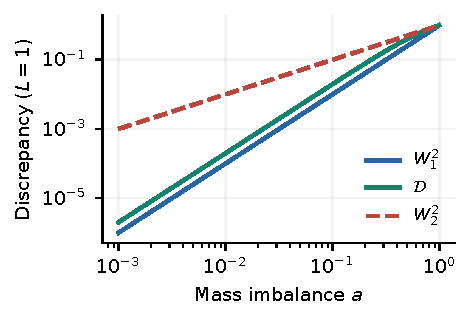
\includegraphics[width=.48\textwidth]{figures/transport_bounds.pdf}
\caption{Exact two-point example from Appendix~\ref{app:proofs}. The midpoint discrepancy controls $W_1^2$ but need not control $W_2^2$ by a universal linear constant. Curves are analytic, not learned-model estimates.}\label{fig:bounds}\end{figure}
\subsection{Historical Additional-Geometry Pilots}
The following historical runs use the legacy metric estimator and one training seed. Its kernel was fitted from generated and target points, and test metrics were monitored during development. We report final steps only, but historical tuning exposure remains. Values are exploratory and must not be pooled with the new fixed-kernel, three-seed tables. Paired-source tasks were adapted to target-only generation by retaining $x_1$; therefore the maze and hyperbolic rows do not reproduce the original source-to-target transport experiment.
Table~\ref{tab:legacy-extra} records all matching historical final-step runs, including repeated configurations rather than selecting the best observed result.
\begin{table}[t]\caption{Historical additional-geometry pilots with their original estimator. Repeated task/method rows are separate configurations; these values are not comparable to the new fixed-kernel table.}\label{tab:legacy-extra}\centering\small\begin{tabular}{@{}llrrrr@{}}\toprule
Task & Method & Dimension & Steps & Legacy MMD$^2$ & Legacy sym. NN \\
\midrule
hyperbolic & Light RFM & 2 & 2000 & 0.0151 & 0.0269 \\
hyperbolic & R-MGM & 2 & 2000 & 0.0108 & 0.0089 \\
maze3v2 & Light RFM & 3 & 500 & 0.1210 & 0.1473 \\
maze3v2 & R-MGM & 3 & 500 & 0.2446 & 0.1293 \\
maze3v2 & R-MGM & 3 & 500 & 0.0009 & 0.0052 \\
maze4v2 & Light RFM & 3 & 500 & 0.0613 & 0.1321 \\
maze4v2 & R-MGM & 3 & 500 & 0.0050 & 0.0078 \\
simple\_bunny & Light RFM & 3 & 500 & 0.5121 & 0.3097 \\
simple\_bunny & R-MGM & 3 & 500 & 0.0023 & 0.0051 \\
wrapped\_spd & Light RFM & 3 & 2000 & 0.0051 & 0.1122 \\
wrapped\_spd & R-MGM & 3 & 2000 & 0.0096 & 0.1144 \\
wrapped\_torus & Light RFM & 5 & 2000 & 0.1912 & 0.5299 \\
wrapped\_torus & R-MGM & 5 & 2000 & 0.0007 & 0.1218 \\
wrapped\_spd & Light RFM & 6 & 1000 & 0.0101 & 0.3962 \\
wrapped\_spd & Light RFM & 10 & 1000 & 0.0067 & 0.7417 \\
wrapped\_spd & R-MGM & 6 & 1000 & 0.0296 & 0.4868 \\
wrapped\_spd & R-MGM & 6 & 1000 & 0.0087 & 0.4137 \\
wrapped\_spd & R-MGM & 10 & 1000 & 0.0169 & 0.8048 \\
wrapped\_torus & Light RFM & 10 & 1000 & 0.4044 & 1.6642 \\
wrapped\_torus & Light RFM & 20 & 1000 & 0.4979 & 3.6284 \\
wrapped\_torus & R-MGM & 10 & 1000 & 0.0010 & 0.3639 \\
wrapped\_torus & R-MGM & 20 & 1000 & 0.0010 & 0.7266 \\
\bottomrule\end{tabular}\end{table}
Wrapped-SPD vector dimensions 3, 6, 10 correspond to matrix sizes 2, 3, 4. They are synthetic data, not EEG covariance models. The high-dimensional torus pilots cover dimensions 5, 10 and 20 only; they are not the full author scaling sweep.
Figure~\ref{fig:extra-volcano} shows the fixed-seed comparison for Volcano.
\begin{figure*}[t]\centering
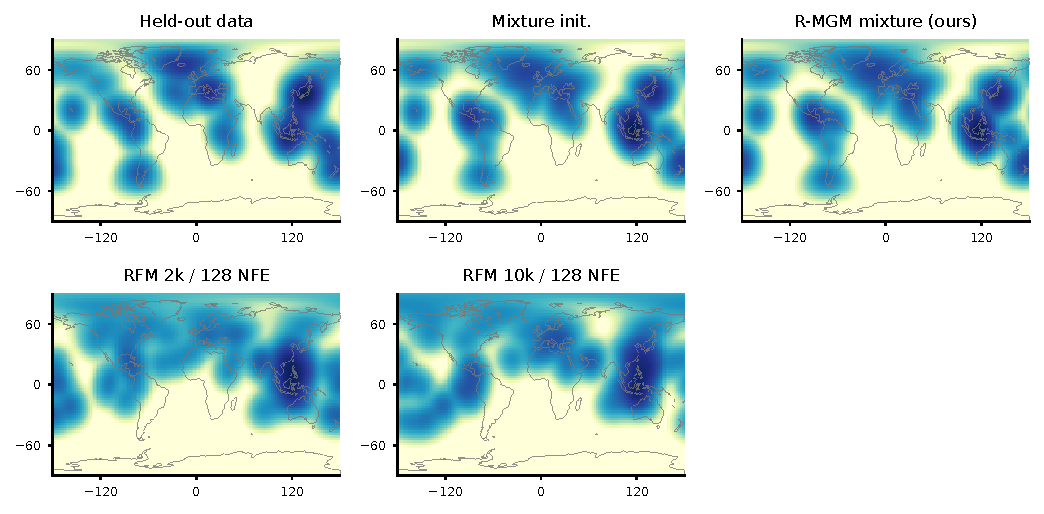
\includegraphics[width=\textwidth]{figures/volcano_comparison.pdf}
\caption{Volcano: fixed test target and training seed 0. Columns are labeled with their generator or flow training budget. Common-bandwidth sample KDEs use the same scale within this figure; these are not likelihood plots.}\label{fig:extra-volcano}\end{figure*}
Figure~\ref{fig:extra-earthquake} shows the fixed-seed comparison for Earthquake.
\begin{figure*}[t]\centering
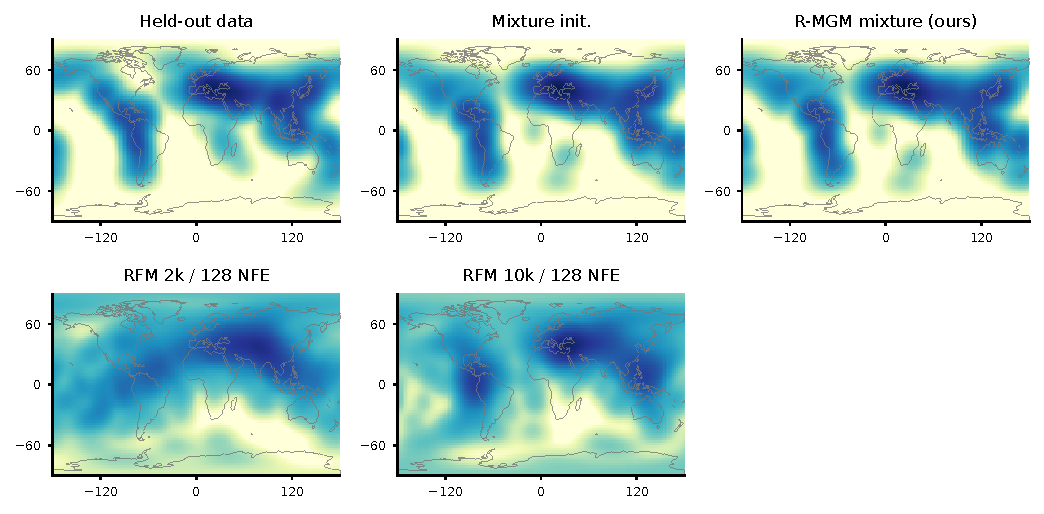
\includegraphics[width=\textwidth]{figures/earthquake_comparison.pdf}
\caption{Earthquake: fixed test target and training seed 0. Columns are labeled with their generator or flow training budget. Common-bandwidth sample KDEs use the same scale within this figure; these are not likelihood plots.}\label{fig:extra-earthquake}\end{figure*}
Figure~\ref{fig:extra-flood} shows the fixed-seed comparison for Flood.
\begin{figure*}[t]\centering
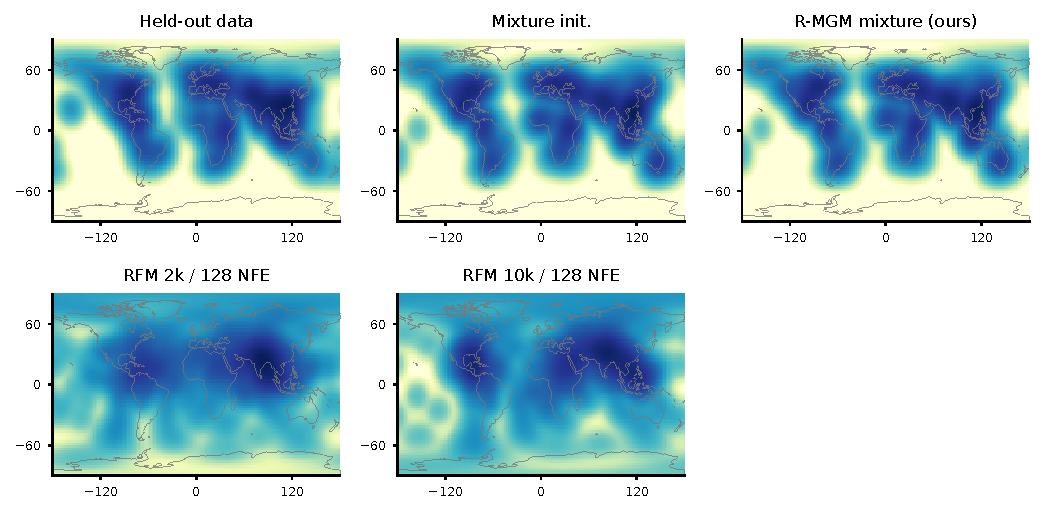
\includegraphics[width=\textwidth]{figures/flood_comparison.pdf}
\caption{Flood: fixed test target and training seed 0. Columns are labeled with their generator or flow training budget. Common-bandwidth sample KDEs use the same scale within this figure; these are not likelihood plots.}\label{fig:extra-flood}\end{figure*}
Figure~\ref{fig:extra-fire} shows the fixed-seed comparison for Fire.
\begin{figure*}[t]\centering
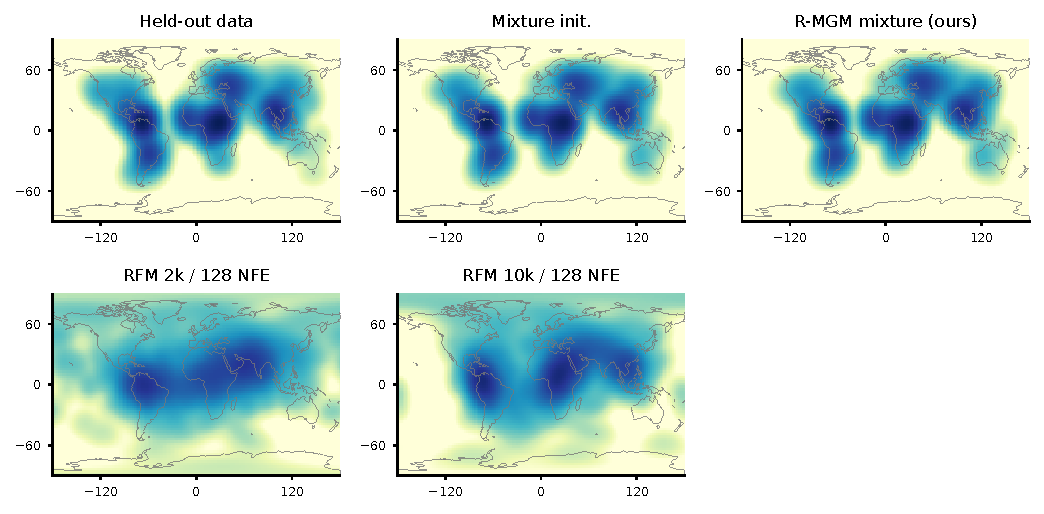
\includegraphics[width=\textwidth]{figures/fire_comparison.pdf}
\caption{Fire: fixed test target and training seed 0. Columns are labeled with their generator or flow training budget. Common-bandwidth sample KDEs use the same scale within this figure; these are not likelihood plots.}\label{fig:extra-fire}\end{figure*}
Figure~\ref{fig:extra-general} shows the fixed-seed comparison for General.
\begin{figure*}[t]\centering
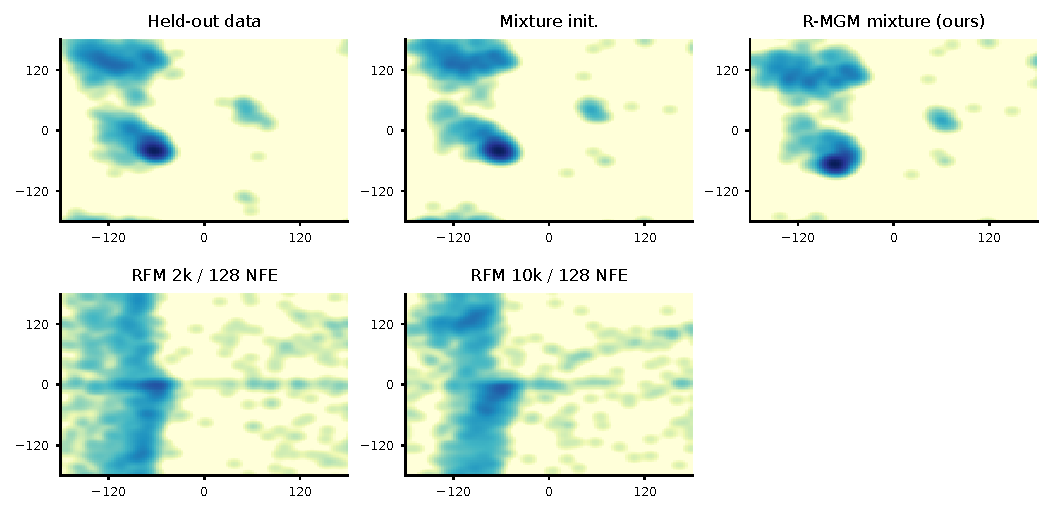
\includegraphics[width=\textwidth]{figures/general_comparison.pdf}
\caption{General: fixed test target and training seed 0. Columns are labeled with their generator or flow training budget. Common-bandwidth sample KDEs use the same scale within this figure; these are not likelihood plots.}\label{fig:extra-general}\end{figure*}
Figure~\ref{fig:extra-glycine} shows the fixed-seed comparison for Glycine.
\begin{figure*}[t]\centering
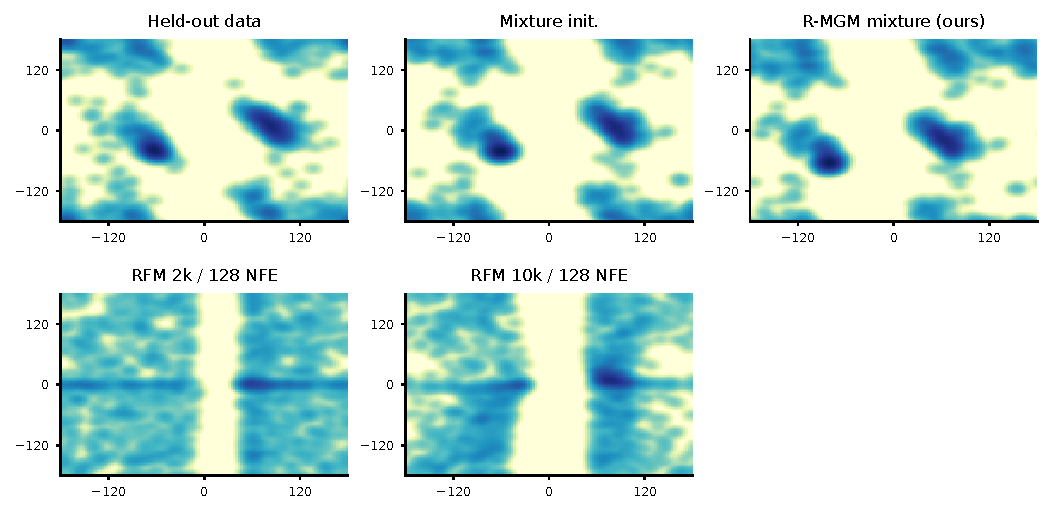
\includegraphics[width=\textwidth]{figures/glycine_comparison.pdf}
\caption{Glycine: fixed test target and training seed 0. Columns are labeled with their generator or flow training budget. Common-bandwidth sample KDEs use the same scale within this figure; these are not likelihood plots.}\label{fig:extra-glycine}\end{figure*}
Figure~\ref{fig:extra-proline} shows the fixed-seed comparison for Proline.
\begin{figure*}[t]\centering
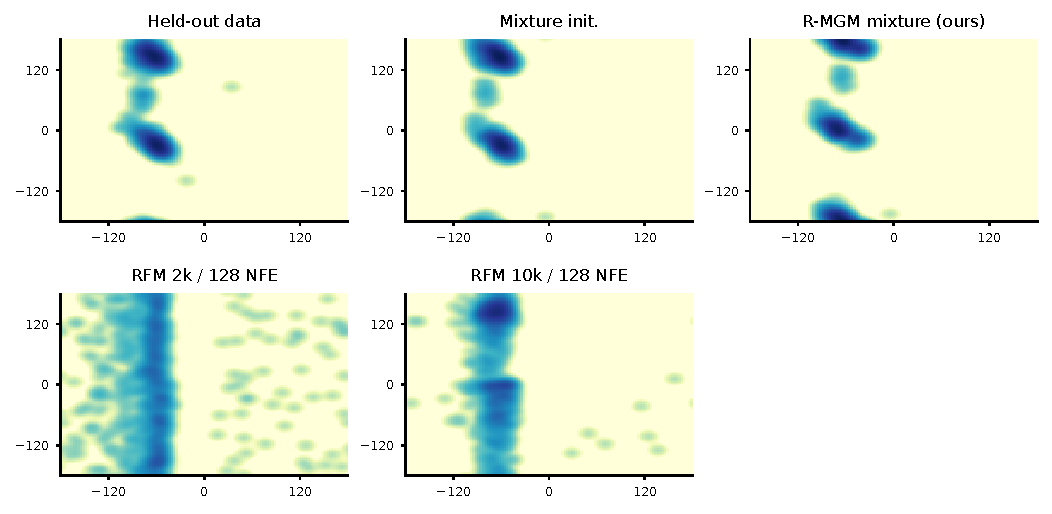
\includegraphics[width=\textwidth]{figures/proline_comparison.pdf}
\caption{Proline: fixed test target and training seed 0. Columns are labeled with their generator or flow training budget. Common-bandwidth sample KDEs use the same scale within this figure; these are not likelihood plots.}\label{fig:extra-proline}\end{figure*}
Figure~\ref{fig:extra-prepro} shows the fixed-seed comparison for Pre-Pro.
\begin{figure*}[t]\centering
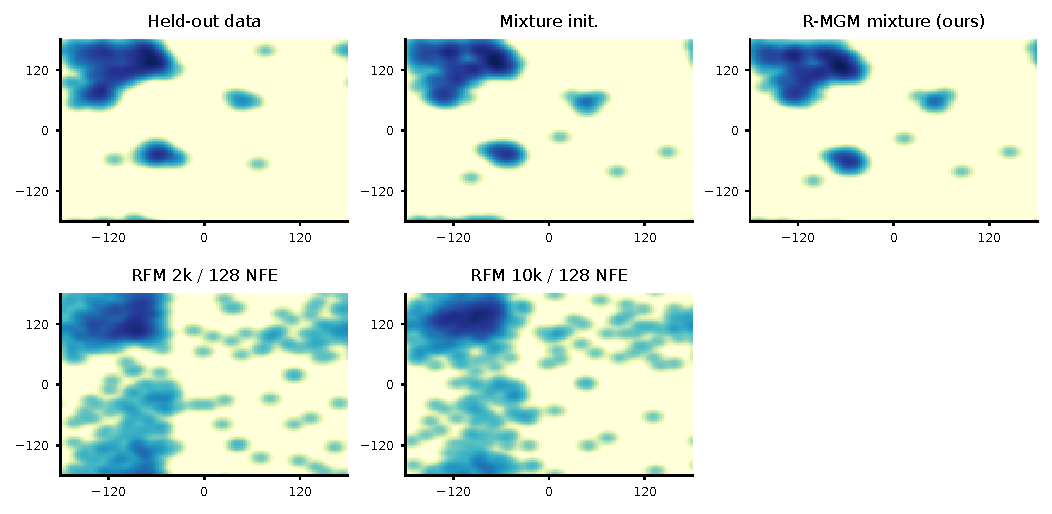
\includegraphics[width=\textwidth]{figures/prepro_comparison.pdf}
\caption{Pre-Pro: fixed test target and training seed 0. Columns are labeled with their generator or flow training budget. Common-bandwidth sample KDEs use the same scale within this figure; these are not likelihood plots.}\label{fig:extra-prepro}\end{figure*}
Figure~\ref{fig:extra-rna} shows the fixed-seed comparison for RNA (7D).
\begin{figure*}[t]\centering
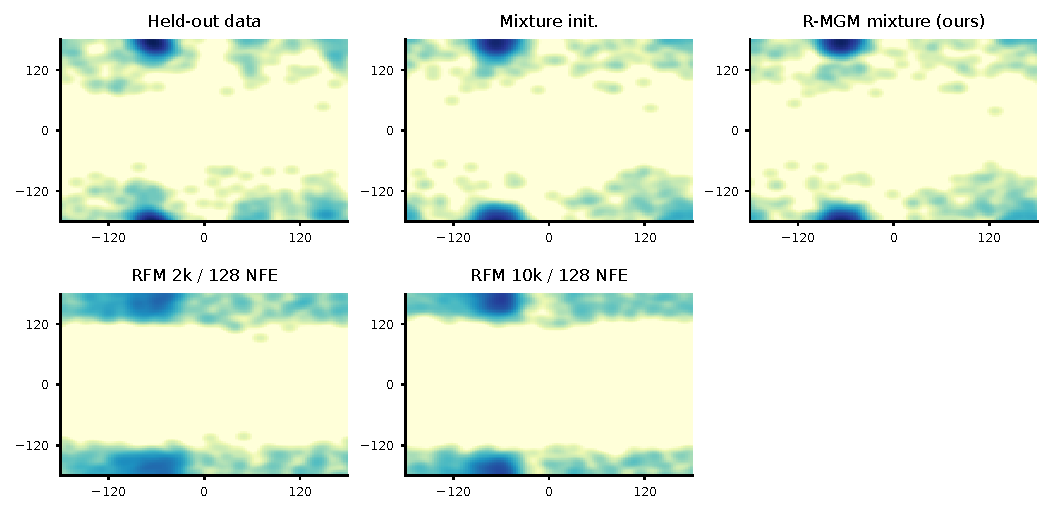
\includegraphics[width=\textwidth]{figures/rna_comparison.pdf}
\caption{RNA (7D): fixed test target and training seed 0. Columns are labeled with their generator or flow training budget. Common-bandwidth sample KDEs use the same scale within this figure; these are not likelihood plots.}\label{fig:extra-rna}\end{figure*}
\subsection{Final-Checkpoint Exploratory Mesh Results}
Each row is a single seed-0 model trained for 800 iterations. Values average three generated draws against the same 1,024 held-out targets. The plus/minus below is Monte Carlo sample SD, not training-seed variation. All kernels and coverage radii use a fixed training reference. The targets retain historical test exposure; final-checkpoint reevaluation does not erase it.
Table~\ref{tab:mesh} gives the final-checkpoint surface results.
\begin{table}[t]\caption{Exploratory mesh models: means and Monte Carlo SD over three draws from a single trained model per row. These are ambient sample metrics, not intrinsic likelihoods.}\label{tab:mesh}\centering\small\begin{tabular}{@{}llrrrr@{}}\toprule
Target & Generator & MMD$^2\times10^3$ & Ambient sym. NN & Coverage & Mean feasibility \\
\midrule
bunny10 & Projected mixture & $1.019\pm0.298$ & $0.043\pm0.000$ & $0.384\pm0.017$ & $2.8e-09$ \\
bunny10 & Soft sphere map & $33.905\pm0.992$ & $0.085\pm0.000$ & $0.248\pm0.012$ & $2.9e-09$ \\
bunny10 & Sphere-map mixture & $1.321\pm0.570$ & $0.042\pm0.000$ & $0.383\pm0.005$ & $3.1e-09$ \\
bunny100 & Projected mixture & $1.586\pm0.503$ & $0.063\pm0.001$ & $0.321\pm0.007$ & $3.2e-09$ \\
bunny100 & Soft sphere map & $75.212\pm7.842$ & $0.084\pm0.002$ & $0.161\pm0.007$ & $3.7e-09$ \\
bunny100 & Sphere-map mixture & $2.381\pm0.576$ & $0.056\pm0.001$ & $0.317\pm0.020$ & $3.1e-09$ \\
bunny50 & Projected mixture & $0.524\pm0.208$ & $0.043\pm0.001$ & $0.429\pm0.017$ & $2.7e-09$ \\
bunny50 & Soft sphere map & $53.416\pm2.984$ & $0.111\pm0.002$ & $0.158\pm0.014$ & $3.2e-09$ \\
bunny50 & Sphere-map mixture & $1.156\pm0.096$ & $0.048\pm0.001$ & $0.375\pm0.005$ & $2.9e-09$ \\
spot10 & Projected mixture & $0.751\pm0.398$ & $0.027\pm0.001$ & $0.453\pm0.035$ & $1.8e-09$ \\
spot10 & Soft sphere map & $47.778\pm1.717$ & $0.093\pm0.001$ & $0.189\pm0.004$ & $2.4e-09$ \\
spot10 & Sphere-map mixture & $1.167\pm0.601$ & $0.028\pm0.001$ & $0.444\pm0.013$ & $2.1e-09$ \\
spot100 & Projected mixture & $1.212\pm0.210$ & $0.052\pm0.002$ & $0.308\pm0.029$ & $2.8e-09$ \\
spot100 & Soft sphere map & $17.464\pm2.354$ & $0.061\pm0.002$ & $0.168\pm0.021$ & $2.8e-09$ \\
spot100 & Sphere-map mixture & $1.027\pm0.152$ & $0.047\pm0.001$ & $0.268\pm0.009$ & $2.8e-09$ \\
spot50 & Projected mixture & $1.897\pm0.666$ & $0.042\pm0.000$ & $0.388\pm0.008$ & $3.0e-09$ \\
spot50 & Soft sphere map & $35.720\pm3.309$ & $0.082\pm0.001$ & $0.153\pm0.010$ & $2.7e-09$ \\
spot50 & Sphere-map mixture & $2.516\pm0.586$ & $0.041\pm0.000$ & $0.385\pm0.005$ & $2.7e-09$ \\
\bottomrule\end{tabular}\end{table}
Surface feasibility measures mean distance to a second closest-point projection. It is not an intrinsic density metric or a certificate of bijective parameterization. The soft map interpolates radii from mesh-vertex directions and then projects; it is not the separate ray-intersection utility.
Figure~\ref{fig:surface-bunny10} gives the full parameterization comparison for bunny10.
\begin{figure*}[t]\centering
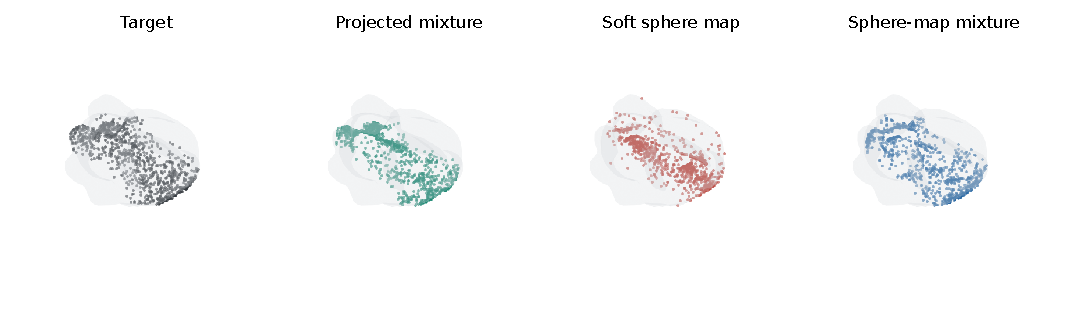
\includegraphics[width=\textwidth]{figures/bunny10_surface.pdf}
\caption{bunny10: one fixed seed-0 final checkpoint per variant, common cameras and 1,024 points. The loss is a local projection surrogate, not the spectral-path construction.}\label{fig:surface-bunny10}\end{figure*}
Figure~\ref{fig:surface-bunny50} gives the full parameterization comparison for bunny50.
\begin{figure*}[t]\centering
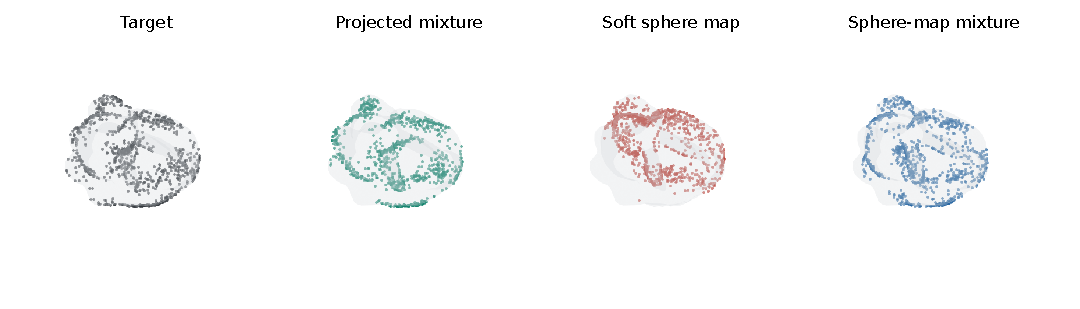
\includegraphics[width=\textwidth]{figures/bunny50_surface.pdf}
\caption{bunny50: one fixed seed-0 final checkpoint per variant, common cameras and 1,024 points. The loss is a local projection surrogate, not the spectral-path construction.}\label{fig:surface-bunny50}\end{figure*}
Figure~\ref{fig:surface-bunny100} gives the full parameterization comparison for bunny100.
\begin{figure*}[t]\centering
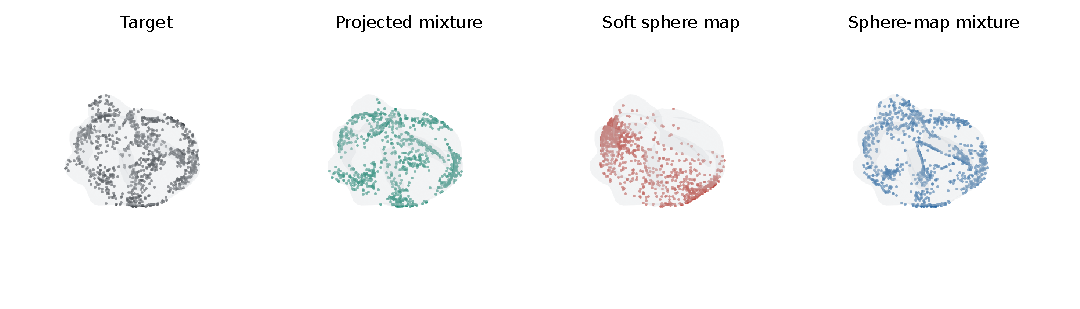
\includegraphics[width=\textwidth]{figures/bunny100_surface.pdf}
\caption{bunny100: one fixed seed-0 final checkpoint per variant, common cameras and 1,024 points. The loss is a local projection surrogate, not the spectral-path construction.}\label{fig:surface-bunny100}\end{figure*}
Figure~\ref{fig:surface-spot10} gives the full parameterization comparison for spot10.
\begin{figure*}[t]\centering
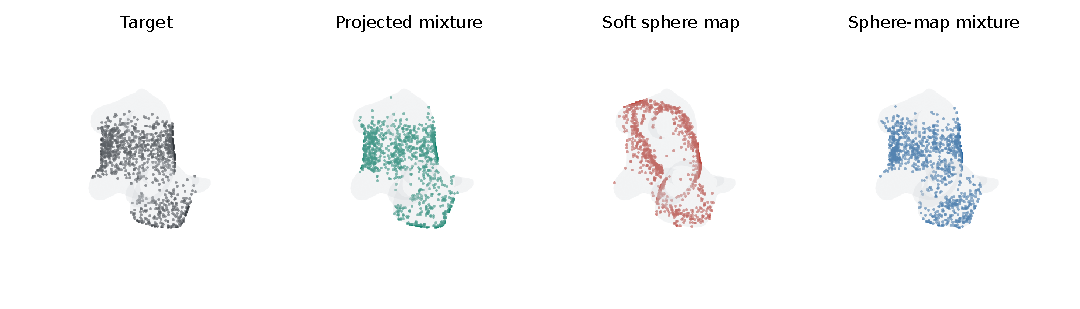
\includegraphics[width=\textwidth]{figures/spot10_surface.pdf}
\caption{spot10: one fixed seed-0 final checkpoint per variant, common cameras and 1,024 points. The loss is a local projection surrogate, not the spectral-path construction.}\label{fig:surface-spot10}\end{figure*}
Figure~\ref{fig:surface-spot50} gives the full parameterization comparison for spot50.
\begin{figure*}[t]\centering
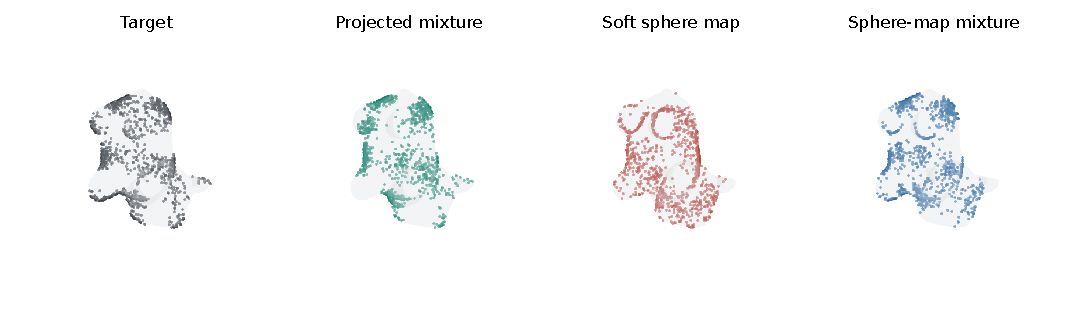
\includegraphics[width=\textwidth]{figures/spot50_surface.pdf}
\caption{spot50: one fixed seed-0 final checkpoint per variant, common cameras and 1,024 points. The loss is a local projection surrogate, not the spectral-path construction.}\label{fig:surface-spot50}\end{figure*}
Figure~\ref{fig:surface-spot100} gives the full parameterization comparison for spot100.
\begin{figure*}[t]\centering
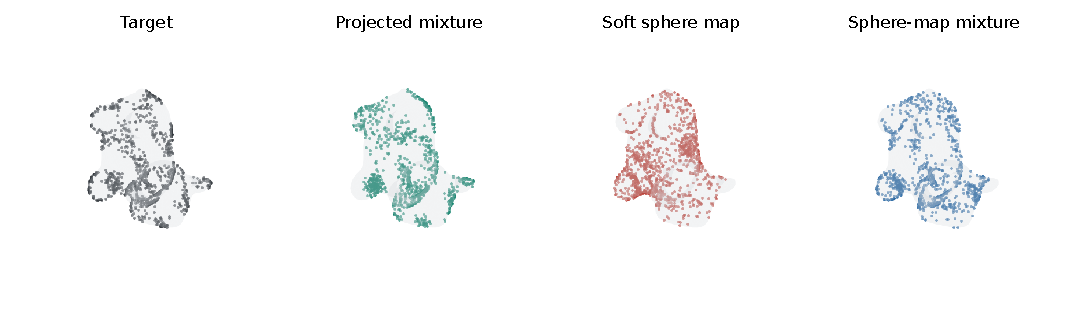
\includegraphics[width=\textwidth]{figures/spot100_surface.pdf}
\caption{spot100: one fixed seed-0 final checkpoint per variant, common cameras and 1,024 points. The loss is a local projection surrogate, not the spectral-path construction.}\label{fig:surface-spot100}\end{figure*}


\clearpage
\section{Scope Compared with the RFM Benchmark}
\label{app:inventory}
The evaluation includes the Earth event and protein/RNA angle tasks associated with the RFM code. They are distribution-learning tasks, not hazard prediction or molecular simulation. The closed-surface targets are positive-eigenfunction distributions on Bunny and Spot with target indices $10,50,100$. This target index differs from the number of spectral eigenfunctions used to construct an RFM path. A projection surrogate does not use spectral paths merely because its target data were generated from eigenfunctions.

Original real-data RFM configurations allow one million updates for Earth and protein/RNA. The existing original-code queue did not complete such runs; its presence is not evidence of completion. Controlled RFM rows use their own recorded architecture and budget. Small synthetic SPD cases are distinct from real EEG covariances: the $6\times6$, $25\times25$, and $59\times59$ EEG experiments are not reproduced here. Sample MMD is never substituted into a likelihood table.

Table~\ref{tab:benchmark-scope} records the distinction between shared data and a faithful reproduction of a published experiment.
\begin{table}[t]
\caption{Coverage of RFM experiment families. Using a reference target dataset does not imply matching its original model, geometry implementation, training budget, or likelihood evaluation.}
\label{tab:benchmark-scope}
\centering\small
\begin{tabular}{@{}p{.25\textwidth}p{.24\textwidth}p{.44\textwidth}@{}}
\toprule
Reference family & Present evidence & Important difference \\
\midrule
Earth data on $\mathbb S^2$ & Four controlled tasks, three seeds & Smaller RFM, 2k/10k updates; sample metrics, not author-budget NLL \\
Protein torsions on $\mathbb T^2$ & Four controlled tasks, three seeds & Row split; raw-angle primary fields; initialization and objective controls \\
RNA on $\mathbb T^7$ & Controlled task, three seeds & Local preprocessing count; same limited flow budget \\
Bunny and Spot surfaces & Six targets, three generator variants & One historical seed; projected-path surrogate; ambient sample metrics \\
Manifold with boundary / maze & Historical target-only pilot & Adapted source law and local projection; not the original transport task \\
High-dimensional scaling & Historical tori in dimensions 5, 10, 20 & Partial sweep, one seed, legacy estimator \\
Hyperbolic / additional geometries & Historical pilot and geometry checks & Target-only adaptation; approximate path velocity \\
Real EEG SPD covariances & Not completed & Synthetic small SPD pilots do not reproduce EEG results \\
\bottomrule
\end{tabular}
\end{table}

\section{Comparison of the Learning Constructions}
\label{app:comparisons}
Table~\ref{tab:constructions} contrasts the learned objects and training signals.
\begin{table}[t]
\caption{Relationship between geometric generative constructions. One-step inference alone is shared by several prior approaches.}
\label{tab:constructions}
\centering\small
\begin{tabular}{@{}p{.19\textwidth}p{.23\textwidth}p{.27\textwidth}p{.22\textwidth}@{}}
\toprule
Construction & Learned object & Defining training signal & Inference \\
\midrule
RFM \citep{chen2024general} & Time-dependent tangent field & Conditional geometric path-velocity regression & Integrate a learned field \\
Riemannian consistency / flow maps \citep{cheng2025rcm,davis2026gfm,woo2026rmf,zhong2026rmf} & Direct or two-time geometric map & Consistency, average-velocity, or flow-map identities & One or a few map evaluations \\
Intrinsic drifting / Wasserstein methods \citep{estebancasadevall2026kgdm,nurgulan2026rwflow,li2026rwgf} & Amortized generator & Kernel- or energy-induced distributional fields & One generator evaluation \\
R-MGM (ours) & Generator and tangent regression critic & Hidden-flip conditional moments at intermediate points & One generator evaluation \\
\bottomrule
\end{tabular}
\end{table}
This taxonomy specifies constructions rather than an empirical ranking. Some consistency methods admit both distillation and from-scratch training; one-step inference and the absence of a teacher alone do not distinguish our proposal. Population identifiability, energy dissipation, finite-horizon particle approximation, and convergence of finite neural training are different claims. They must be checked against the corresponding assumptions of each paper.

In particular, the midpoint critic is evaluated at a symmetrized intermediate location. Updating the generator requires derivatives through the path and its velocity, rather than simply applying the critic as a drift at the generated endpoint. A kernel-based particle update with a stop-gradient regression target implements a different optimization rule. A Wasserstein interpretation of any specific rule would require a first variation and a continuity-equation argument for its training-time dynamics. Our interpolation-current identity proves a distribution-discrepancy bound; it does not establish such an optimization-dynamics equivalence.

\section{Reproducibility and Computational Resources}
\label{app:reproduce}
The accompanying scripts generate tables from recorded machine-readable results and figures from sample arrays. The generated protocol lists commands, seeds, split identifiers, package versions, durations, and checkpoints. New GPU work uses one NVIDIA GeForce RTX 4090. Repeated Monte Carlo evaluations of one checkpoint are distinguished from independent training seeds. The PowerShell build script calls installed MiKTeX PDFLaTeX and BibTeX; unmodified ICML style files accompany the sources.

\paragraph{AI assistance.}
Generative AI tools assisted manuscript drafting, implementation, and internal error checking. They are not components of the evaluated generative models. The internal reviews are automated checks, not independent human peer review. Scientific validation and responsibility remain with the human authors.
